\chapter{PROTÓTIPO}
\label{chap:prototipos}

Neste capítulo, apresentam-se três protótipos experimentais desenvolvidos com o propósito de avaliar e validar o fatiamento de rede (\textit{network slicing}) e a garantia de requisitos de Qualidade de Serviço (QoS) sob a ótica do sistema de numeração de resíduos (RNS, do inglês \textit{Residue Number System}). A abordagem adota uma estratégia incremental de validação, cobrindo diferentes níveis de fidelidade de hardware, flexibilidade de prototipagem e eficiência de encaminhamento:

\begin{enumerate}
    \item \textbf{Ambiente em hardware programável (Tofino/freeRtr):} topologia interestadual com enlaces de 10~Gbps e comutadores baseados no circuito integrado Intel Tofino\textregistered, operando sob o \textit{framework} freeRtr, com o objetivo de atestar a capacidade da arquitetura PolKA original em prover garantias de QoS estritamente por meio da seleção de caminhos fim a fim;
    \item \textbf{Ambiente comportamental P4 (BMv2/Mininet):} implementação concebida para validar as extensões da arquitetura SPolKA (\textit{Service PolKA}), elevando a granularidade do fatiamento ao codificar a rota de encaminhamento e a classe de escalonamento em um único rótulo no cabeçalho;
    \item \textbf{Ambiente baseado em contêineres e SO programável (Containerlab/eBPF):} infraestrutura leve orquestrada sobre contêineres Ubuntu, empregando eBPF (\textit{Extended Berkeley Packet Filter}) no plano de dados para executar o encapsulamento, a manipulação de rótulos e o encaminhamento eficiente dos pacotes em ambiente de rede virtualizada.
\end{enumerate}

A coexistência dessas três frentes experimentais fundamenta-se nas características e restrições de cada ecossistema. As operações de plano de dados introduzidas pelo SPolKA preservam a mesma base aritmética do PolKA tradicional, cuja viabilidade em taxa de linha já foi previamente validada em hardware Tofino por \cite{dominicini2021}. Contudo, como o \textit{framework} de controle freeRtr ainda não contempla nativamente as extensões de cabeçalho necessárias para o SPolKA, optou-se pela implementação comportamental em switches BMv2 sobre o emulador Mininet.

Para contornar o problema de inanição (\textit{starvation}) decorrente da política de prioridade estrita (\textit{Strict Priority}) nativa do BMv2, aprimorou-se a arquitetura de enfileiramento com o algoritmo \textit{Weighted Deficit Round-Robin} (WDRR), distribuindo a largura de banda de forma proporcional aos pesos atribuídos a cada fatia. Fundamentando-se na abordagem proposta por \cite{Elbediwy2025}, integrou-se um \textit{Traffic Manager} (TM) customizado em C++ por meio de \textit{software externs}, transferindo os pacotes ao módulo de gerenciamento de tráfego ao término do estágio de \textit{Ingress}. Com isso, o comportamento do ambiente emulado aproxima-se com fidelidade da dinâmica de comutadores de produção.

No plano de controle e borda da rede (\textit{ingress edge}), a classificação de tráfego utiliza o campo DSCP (\textit{Differentiated Services Code Point}) do modelo DiffServ para derivar o mapeamento conjunto de fluxos, rotas e classes de serviço em um identificador único denominado \texttt{routeID} --- prevendo-se, para trabalhos futuros, a adoção dos parâmetros SST (\textit{Slice/Service Type}) e SD (\textit{Slice Differentiator}) do padrão S-NSSAI da arquitetura 5G/6G. 

No núcleo da rede (\textit{core}), o cálculo dos módulos de resíduos em taxa de linha supera as restrições inerentes da linguagem P4 ao reaproveitar os motores de hardware de CRC. Conforme demonstrado na análise de escalabilidade de \cite{dominicini2020}, a sobrecarga de cabeçalho do \texttt{routeID} é determinada pelo produto do diâmetro máximo da topologia (em saltos) por 2~bytes (CRC-16 com suporte a até 4.080 nós de núcleo). Neste trabalho, definiu-se um limite superior de 10 saltos, resultando em um cabeçalho \texttt{routeID} de 20~bytes, particionado conceitualmente para acomodar identificadores de porta de saída (\texttt{portID}) de 13~bits e identificadores de fila (\texttt{qID}) de 3~bits, viabilizando o isolamento de até 8 filas por interface.

O principal diferencial do SPolKA reside na flexibilidade de adaptação: alterações dinâmicas de trajetos e políticas de escalonamento são efetuadas exclusivamente pela reconfiguração pontual do rótulo na borda, mantendo o núcleo da rede totalmente sem estado (\textit{stateless}). 

Nas seções seguintes, detalham-se os requisitos, a topologia, o fluxo de execução e a instrumentação metodológica empregada em cada um dos protótipos desenvolvidos.


----

Neste capítulo, apresentam-se três protótipos desenvolvidos para mitigar o 
desafio de assegurar os requisitos de Qualidade de Serviço (QoS) para distintas 
classes de serviço. O primeiro protótipo consiste em um ambiente experimental que 
emula uma rede interestadual composta por enlaces de 10~Gbps e comutadores 
baseados no circuito integrado Intel Tofino\textregistered. O segundo cenário 
foi concebido no ambiente de emulação Mininet, utilizando switches de software 
baseados na arquitetura comportamental BMv2. Por fim, o terceiro protótipo 
foi implementado a partir de contêineres Ubuntu orquestrados via Containerlab, 
empregando eBPF para a realização do encapsulamento e do encaminhamento 
eficiente dos pacotes.

Para validar a eficácia do fatiamento baseado em RNS, desenvolveram-se três protótipos complementares. O primeiro, em hardware Tofino sob o framework freeRtr\footnote{\url{http://www.freertr.org/}}, atesta a capacidade do \polka original em prover QoS apenas pela seleção de caminhos fim a fim. O segundo foca no \spolka, elevando a granularidade ao codificar rota e escalonamento em um único rótulo. As operações no plano de dados do \spolka são as mesmas do \polka original, que já foi validado em hardware Tofino \cite{dominicini2021}. Para este trabalho, a solução foi implementar o \spolka no switch de software BMv2 (emulado no Mininet), pois o framework freeRtr ainda não suporta as extensões de cabeçalho do \spolka. Para superar a inanição causada pela prioridade estrita nativa do BMv2, aprimorou-se a arquitetura com o algoritmo Weighted Deficit Round-Robin (WDRR), que distribui a banda proporcionalmente aos pesos das fatias \cite{Elbediwy2025}. Baseando-se em \textcite{Elbediwy2025}\footnote{\url{https://github.com/Elbediwy/DR-PIFO_hierarchical_TM_SW.git}}, integrou-se um Traffic Manager (TM) customizado em C++ via software externs, que transferem os pacotes ao TM no final do pipeline de Ingress. Isso alinha a emulação ao comportamento de hardwares de produção (como o Tofino).

Na borda, a classificação usa o campo DSCP (\textit{Differentiated Services Code Point}) do \textit{DiffServ} para mapear fluxos em rotas e classes de serviço num único \routeID. Em trabalhos futuros, planeja-se adotar os parâmetros SST (\textit{Slice/Service Type}) e SD (\textit{Slice Differentiator}) do identificador S-NSSAI. No núcleo, a operação de módulo em taxa de linha contorna as restrições matemáticas do P4 reusando o hardware de CRC. Conforme detalhado na análise de escalabilidade em \cite{dominicini2020}, o tamanho do cabeçalho do \routeID é dado pela multiplicação do número máximo de saltos da topologia por 2 bytes (CRC16 com até 4.080 nós de núcleo). Neste trabalho, adotou-se o número máximo de 10 saltos, um \routeID de 20 bytes, um portID de 13 bits e um \qID de 3 bits (8 filas). O diferencial do \spolka é a migração ágil de rotas e políticas de filas, alterando apenas um rótulo na borda, sem reconfigurar o núcleo. Os experimentos evidenciam como essa adaptação dinâmica torna o \spolka particularmente eficaz para o fatiamento de redes.

\section{PROTÓTIPO 1 - \polka original: Fatiamento com seleção de caminhos}

A topologia PORVIR (Figura \ref{fig:porvir_rede}) é composta por quatro nós implementados em switches programáveis Tofino. Para avaliar individualmente os caminhos, configuraram se três túneis \polka. Inicialmente, caracterizou-se o desempenho de cada caminho da rede em termos de latência, vazão média e retransmissões, conforme a Tabela 3a. As medições de tráfego TCP ocorreram via iperf3 por 60 minutos para cada caminho, com amostragens a cada 30 s. Adicionalmente, o tempo de resposta médio (RTT) foi aferido com a ferramenta ping (amostras de 1 s) por 60 minutos. Os resultados mostram que o caminho VIX–RJ–SP apresenta desempenho significativamente superior, com vazão 46 vezes maior, menor atraso e menos retransmissões.

\begin{figure}[htbp]
\centering
\captionsetup{justification=centering}

    \begin{subfigure}[b]{0.41\linewidth}
        \centering
        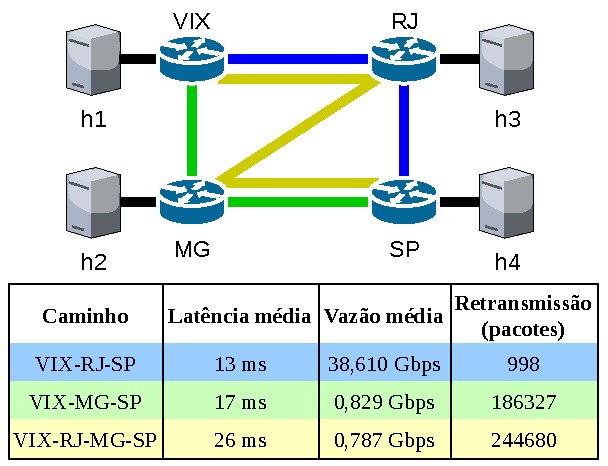
\includegraphics[width=\linewidth]{figuras/Porvir - Tabela e Topo.pdf}
        \caption{Métricas por caminho.}
        \label{fig:porvir_rede}
    \end{subfigure}
    \hfill
    \begin{subfigure}[b]{0.57\linewidth}
        \centering
        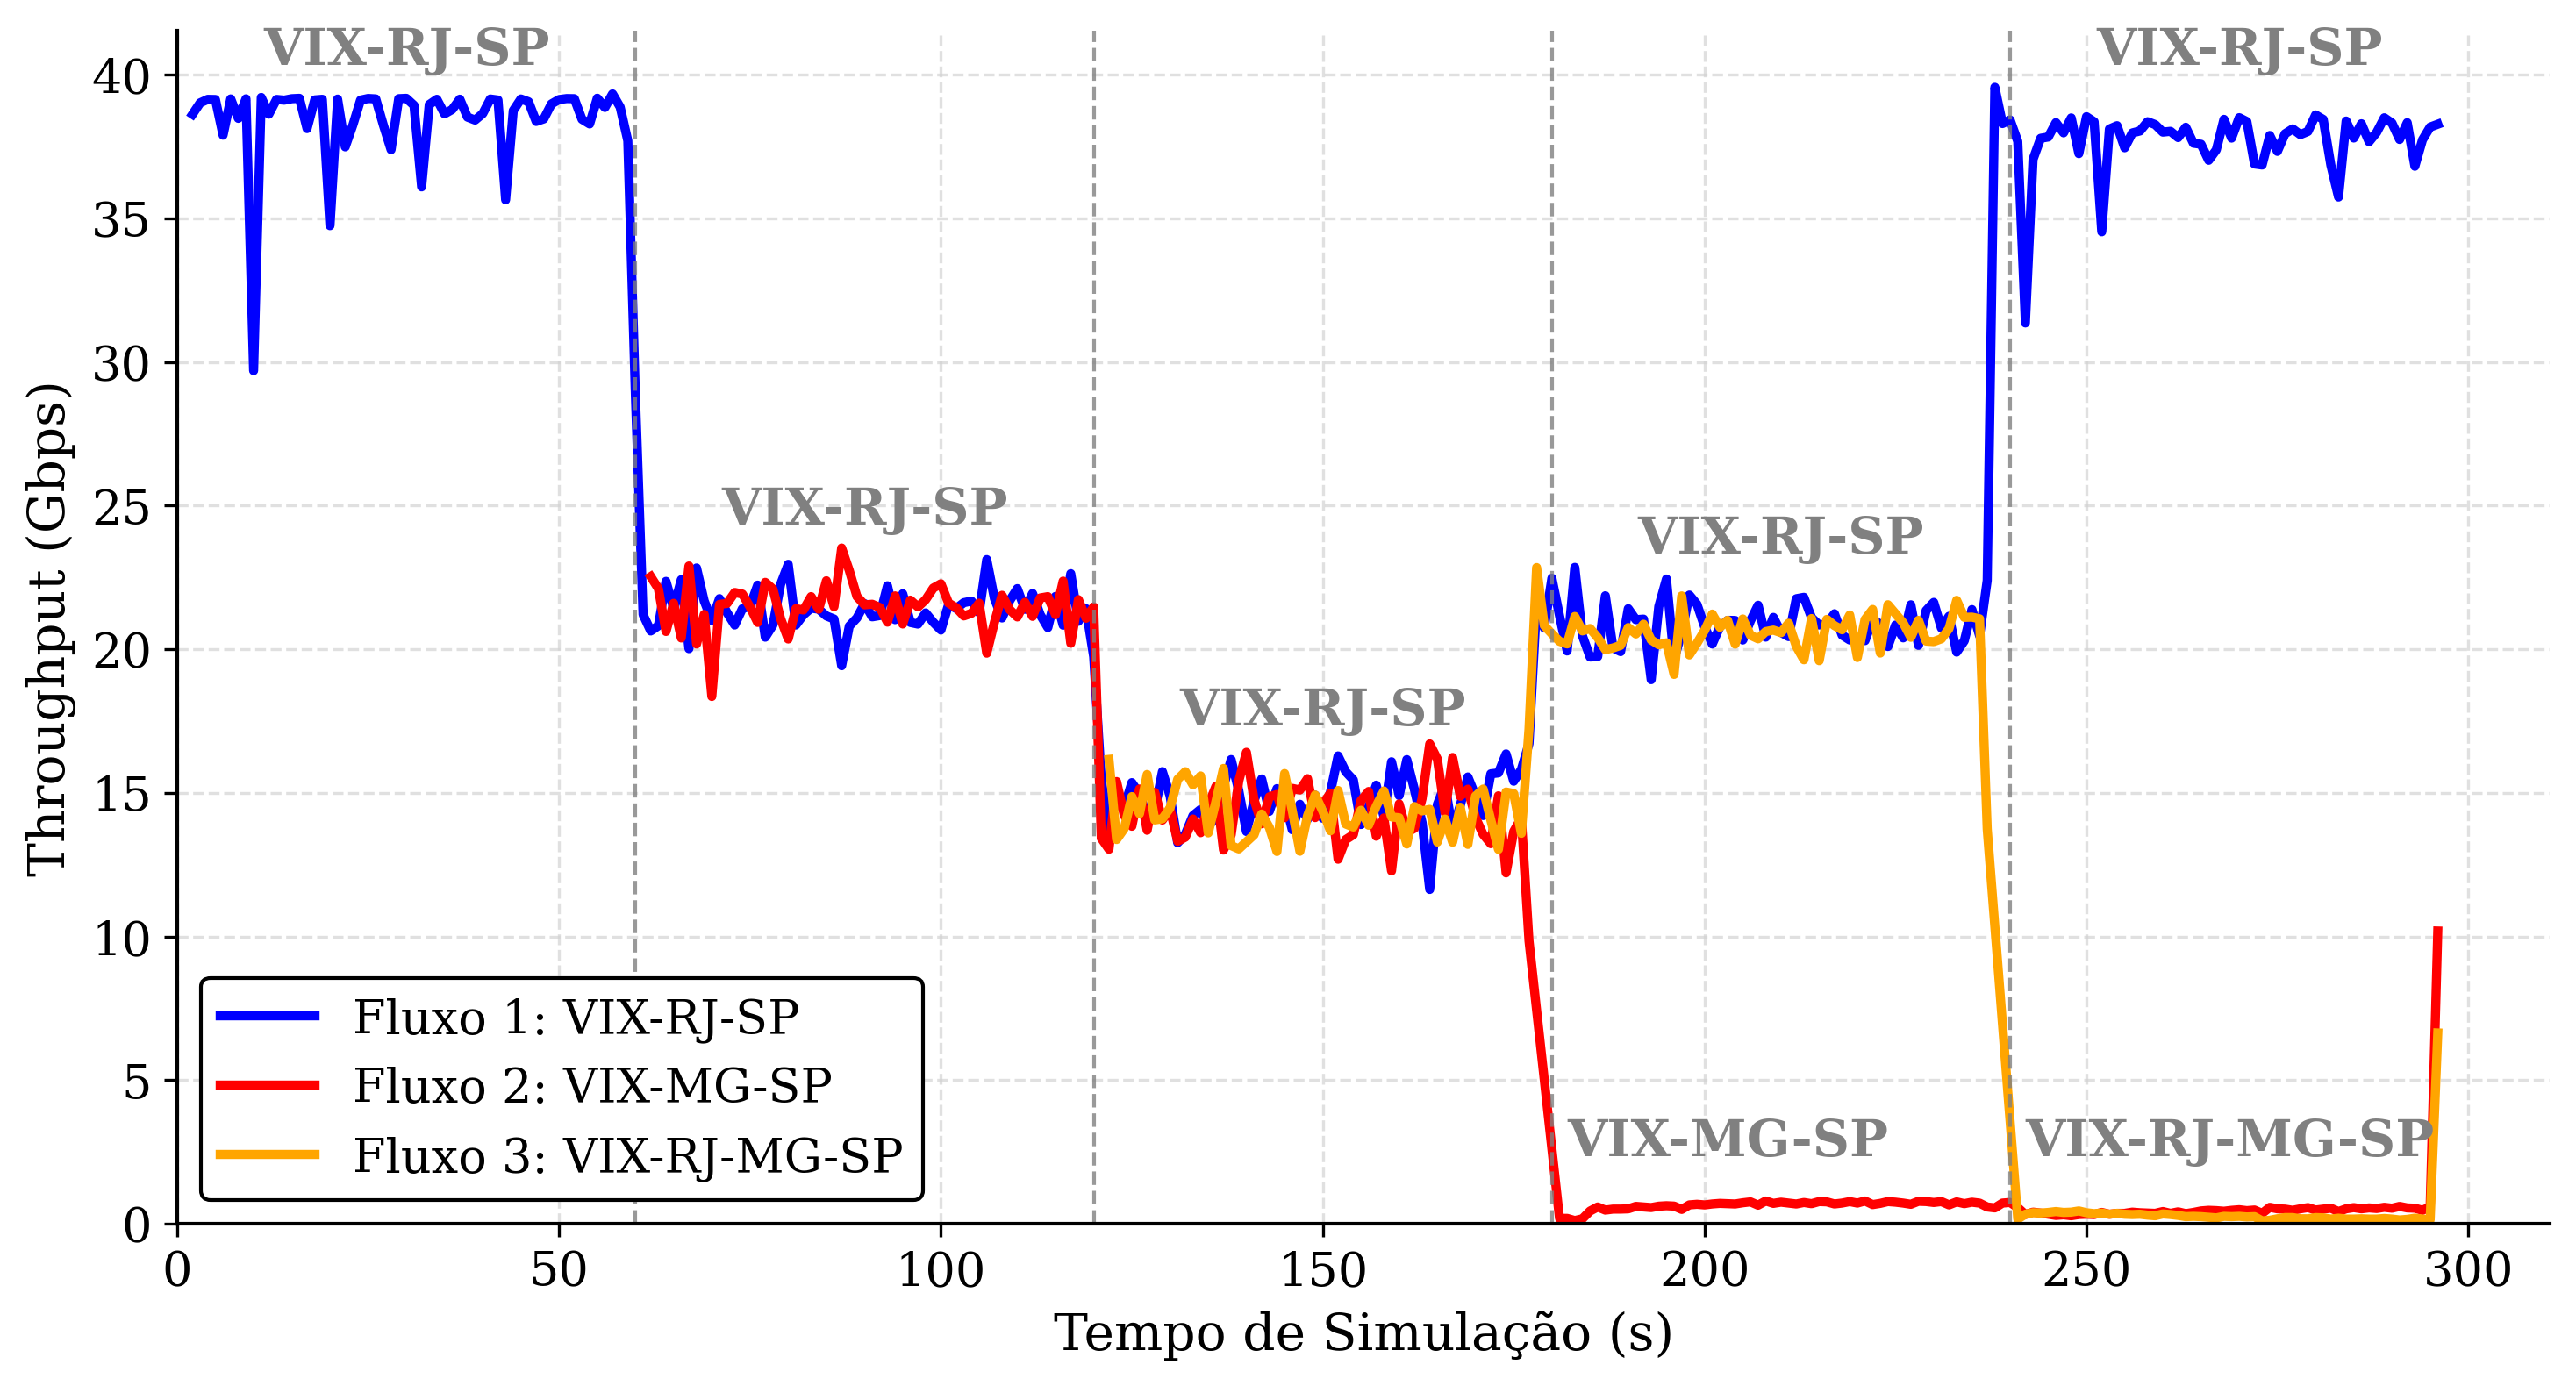
\includegraphics[width=\linewidth]{figuras/grafico_mudanca_caminho_porvir.png}
        \caption{Mudança de caminho.}
        \label{fig:mudanca_caminho_fila}
    \end{subfigure}

\caption{Resultados dos experimentos no testbed nacional Porvir.}
\label{fig:matriz_resultados}
\end{figure}

Após a caracterização, um experimento com três fluxos TCP (via iperf3) no enlace de alta capacidade (VIX–RJ–SP) representou a coexistência de um tráfego de maior prioridade com tráfegos de menor prioridade. Nesse cenário, cada fluxo atua como uma fatia de rede independente, que recebe recursos isolados e é configurada dinamicamente conforme seus requisitos específicos de \textit{QoS}. A figura \ref{fig:mudanca_caminho_fila} apresenta a vazão coletada ao longo dos eventos, espaçados a cada 60 s. Na fase de competição (0–180 s), a fatia do Fluxo 1 inicia isolada no caminho principal. Aos 60 s e 120 s, as fatias dos Fluxos 2 e 3 são ativadas na mesma rota, compartilhando a banda do enlace. Na fase de migração (180–300 s), evidenciando o isolamento e a adaptação dinâmica, as fatias concorrentes são realocadas para rotas alternativas de menor capacidade: o Fluxo 2 para VIX–MG–SP (aos 180 s) e o Fluxo 3 para VIX–RJ–MG–SP (aos 240 s). Com isso, a fatia do Fluxo 1, mais prioritário, restabelece o uso integral do enlace principal.

\section{PROTÓTIPO 2 - \spolka\: Fatiamento com seleção de caminhos e políticas de filas}

O segundo protótipo foi avaliado em dois cenários de acordo com a topologia da Figura \ref{fig:topologia_polka}: no primeiro, investigou-se exclusivamente o impacto da alteração das políticas de filas, enquanto o segundo analisou a reconfiguração concomitante de rotas e filas. Os enlaces têm capacidades de 10~Mbps com duas filas de prioridade por interface em cada roteador: a \textit{Fila 1}, com reserva de 70\% da largura de banda, e a \textit{Fila 2}, com os 30\% remanescentes. Os fluxos de dados foram gerados usando \textit{iperf3} com protocolo TCP. % com uma vazão nominal de 10~Mbps.
\begin{figure}[htbp]
    \centering
    % --- COLUNA DA ESQUERDA (Imagem Grande) ---
    \begin{subfigure}[t]{0.48\textwidth}
        \centering
        \vspace{0pt} % Truque para forçar o alinhamento no topo
        \fbox{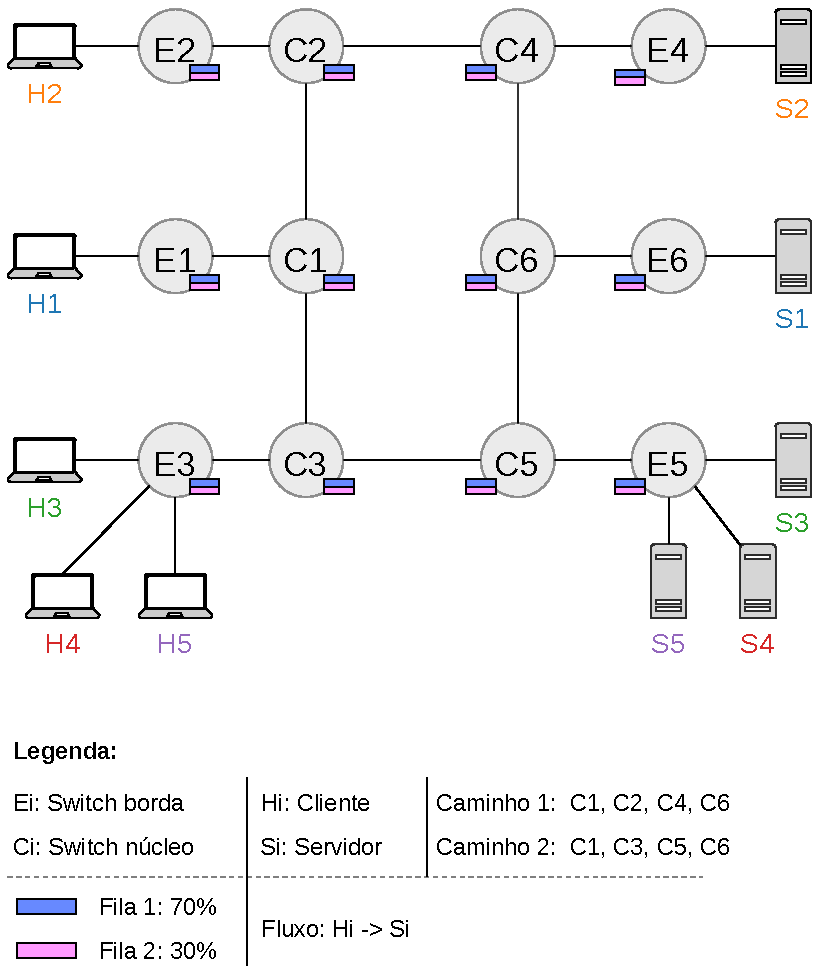
\includegraphics[width=\linewidth]{figuras/topologia - SBRC WPEIF 2026_v4.pdf}}
        \caption{Topologia da rede}
        \label{fig:topologia_polka}
    \end{subfigure}
    \hfill % Joga a outra coluna para o canto direito
    % --- COLUNA DA DIREITA (Duas Imagens Empilhadas) ---
    \begin{minipage}[t]{0.48\textwidth}
        \centering
        \vspace{0pt} % Garante que o topo da minipage alinhe com a esquerda
        
        \begin{subfigure}{\linewidth}
            \centering
            \fbox{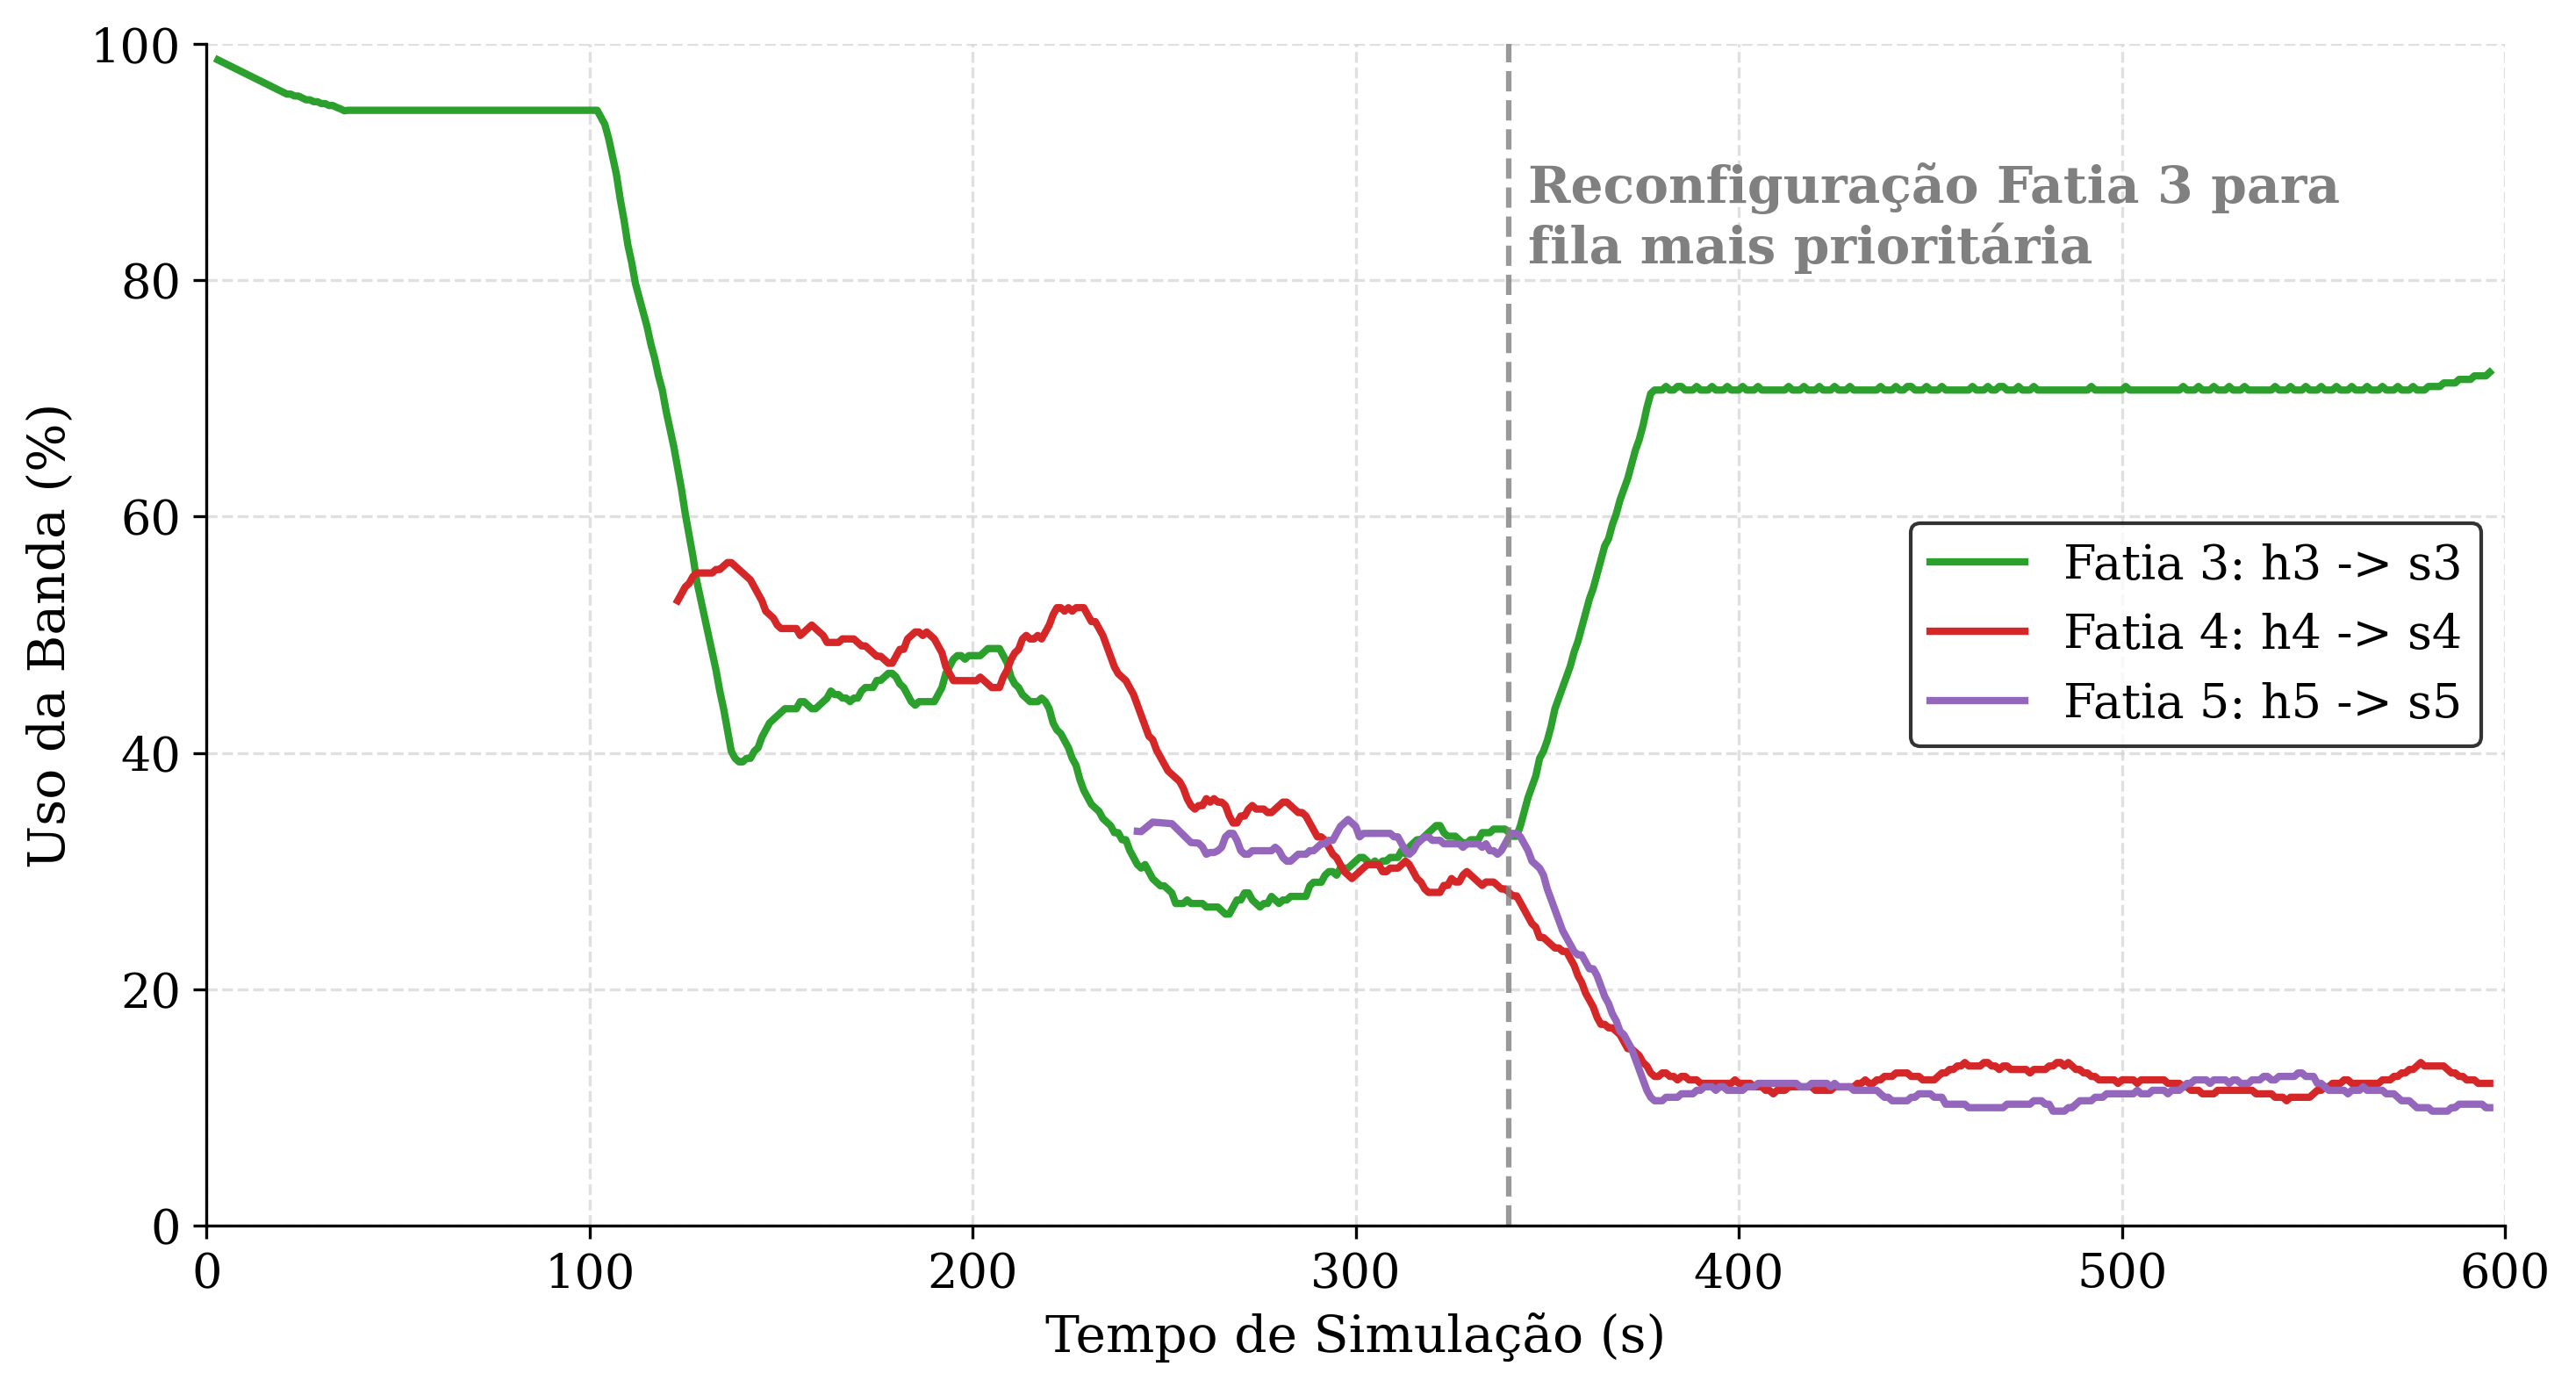
\includegraphics[width=\linewidth]{figuras/grafico_mudanca_fila_polka.png}}
            \caption{Mudança para fila prioritária}
            \label{fig:mininet_mudanca_fila_polka}
        \end{subfigure}
        
        % \vspace{1.0 cm} % Espaço entre as duas da direita
        
        \begin{subfigure}{\linewidth}
            \centering
            \fbox{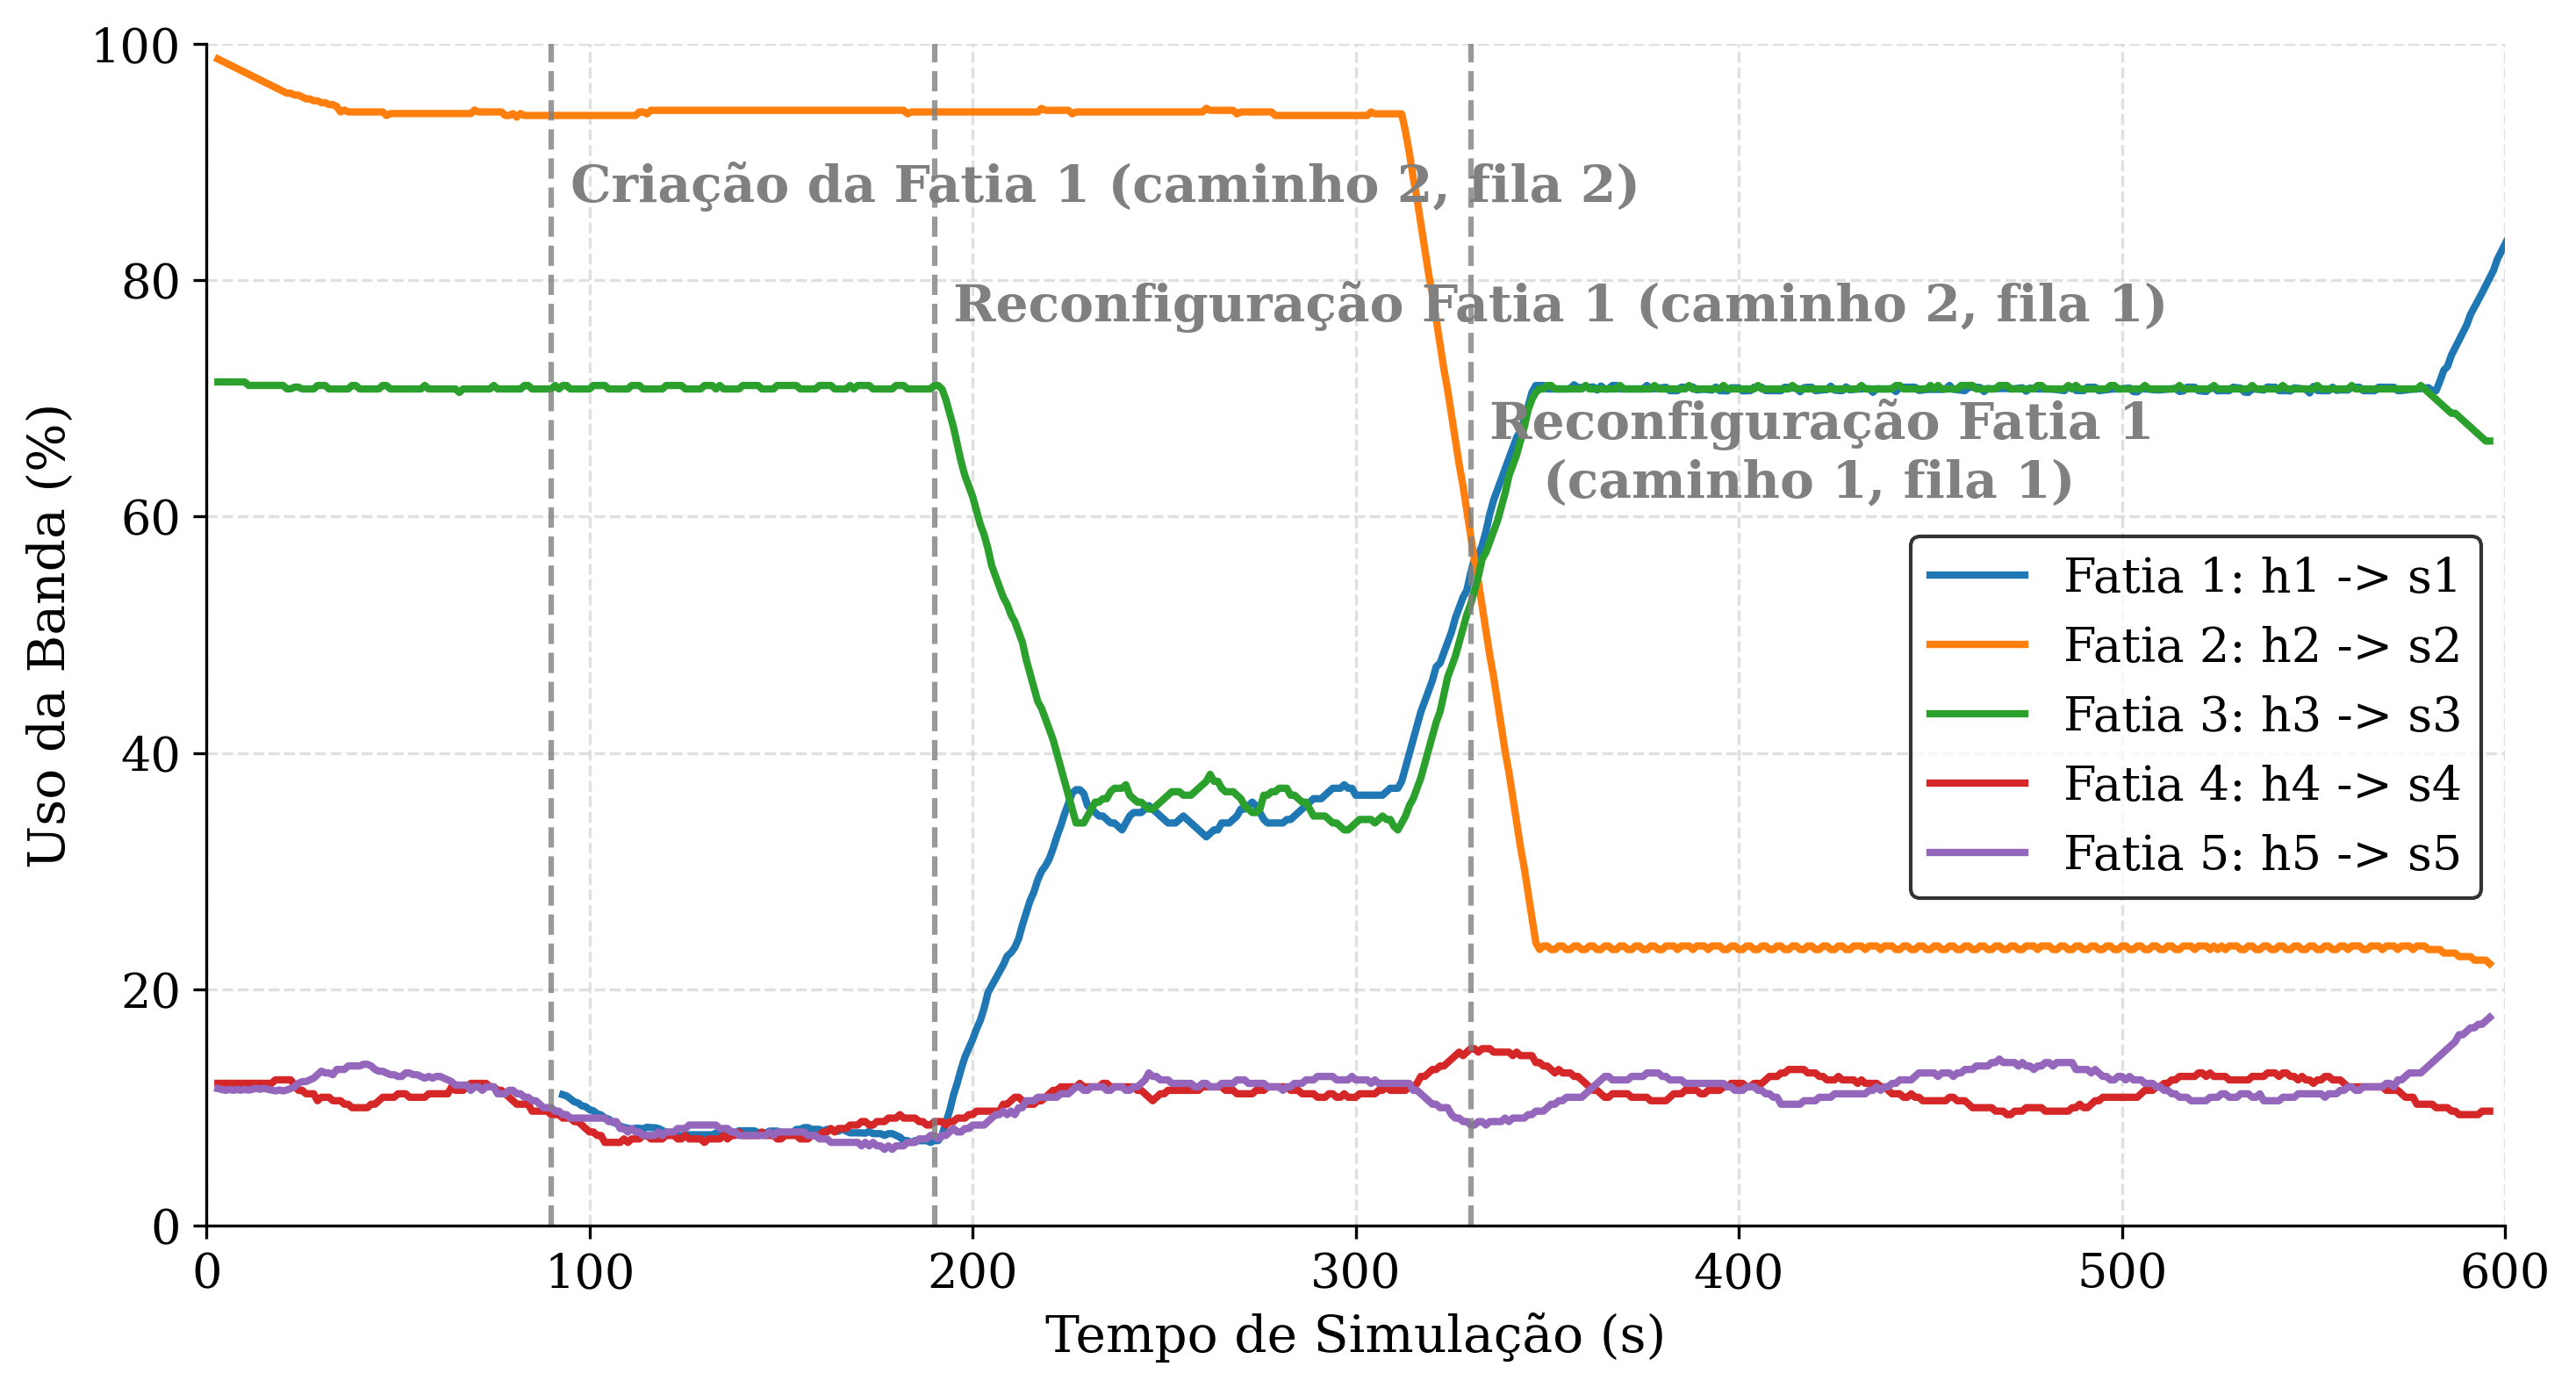
\includegraphics[width=\linewidth]{figuras/grafico_mudanca_caminho_fila_polka.png}}
            \caption{Mudança de caminho e fila}
            \label{fig:mininet_mudanca_caminho_fila}
        \end{subfigure}
    \end{minipage}

    \caption{Alteração de políticas de QoS para fatias de rede com SPolKA.}
    \label{fig:polka_combined}
\end{figure}

No primeiro cenário (Figura \ref{fig:mininet_mudanca_fila_polka}), analisou-se o desempenho de três fatias de rede encaminhadas pela rota $\{C_3, C_5\}$: uma fatia de alta prioridade, representada pelo fluxo $H_3 \rightarrow S_3$, e duas fatias de menor prioridade, representadas pelos fluxos $H_4 \rightarrow S_4$ e $H_5 \rightarrow S_5$. O objetivo foi validar a eficácia do isolamento e da priorização de recursos em condições de saturação de rede.
%
Em $t=0$~s, o fluxo $H_3 \rightarrow S_3$ foi alocado na \textit{Fila 2} em todos os saltos. 
A aplicação do algoritmo WDRR garante que, na ausência de fluxo na fila prioritária, a banda total disponível pode ser compartilhada entre as demais filas.
Posteriormente, em $t=90$~s e $t=180$~s, os fluxos $H_4 \rightarrow S_4$ e $H_5 \rightarrow S_5$ foram configurados, na mesma fila, resultando no compartilhamento equitativo da banda disponível entre as três fatias. 
%. Dado que os nós $C_3$ e $C_5$ constituem o caminho de convergência dos fluxos, a vazão disponível foi fragmentada proporcionalmente entre as três conexões ativas na Fila 2.
%
Finalmente, em $t=270$~s, procedeu-se à reconfiguração do fluxo $H_3 \rightarrow S_3$ para a \textit{Fila 1}, que possui uma reserva estrita de 70\% da largura de banda. Esta reconfiguração visou assegurar o isolamento de desempenho para o tráfego prioritário. Os fluxos remanescentes na Fila 2 (origem $H_4$ e $H_5$) passaram a competir pelos 30\% restantes da capacidade alocada, validando a capacidade do mecanismo de fatiamento em assegurar requisitos de QoS e mitigar interferências entre diferentes classes de serviço. 

% \subsection{Experimento 2 - mudança de caminho e fila}

O segundo cenário (Figura \ref{fig:mininet_mudanca_caminho_fila}) analisa o impacto da reconfiguração dinâmica concomitante de filas e rotas. % para a fatia representada pelo fluxo $H_1 \rightarrow S_1$. 
Em $t=0$~s, foi instanciada uma fatia de rede na rota $\{C_2, C_4\}$ referente ao fluxo $H_2 \rightarrow S_2$ e três fatias na rota $\{C_3, C_5\}$ referentes aos fluxos $H_3 \rightarrow S_3$, $H_4 \rightarrow S_4$ e $H_5 \rightarrow S_5$. A fatia com origem $H_2$ foi alocada na \textit{Fila 2}, ocupando toda a banda disponível, devido à ausência de tráfego concorrente em sua rota. No outro caminho, o fluxo $H_3 \rightarrow S_3$ foi designado à \textit{Fila 1} (prioritária) operando em conjunto com os fluxos $H_4 \rightarrow S_4$ e $H_5 \rightarrow S_5$, alocados na \textit{Fila 2}.
%
Em $t=60$~s, introduziu-se o fluxo $H_1 \rightarrow S_1$ via $\{C_1, C_3, C_5, C_6\}$ na \textit{Fila 2}. Nesse cenário, o tráfego passou a competir pela reserva de 30\% da largura de banda disponível nesta fila com os fluxos $H_4$ e $H_5$. Posteriormente, em $t=180$~s, procedeu-se à reconfiguração do fluxo $H_1 \rightarrow S_1$ para a \textit{Fila 1}, sem alteração de caminho, passando este a compartilhar a reserva de 70\% da banda com o fluxo $H_3 \rightarrow S_3$.
%
Finalmente, em $t=300$~s, realizou-se a migração de rota do fluxo $H_1 \rightarrow S_1$ para o caminho $\{C_1, C_2, C_4, C_6\}$, mantendo-se a configuração na \textit{Fila 1}. Esta reconfiguração de rota mitigou a disputa por recursos críticos: a fatia $H_2 \rightarrow S_2$ passou a ocupar, isoladamente, a reserva da \textit{Fila 2} em seu trajeto, enquanto as fatias prioritárias $H_1 \rightarrow S_1$ e $H_3 \rightarrow S_3$ atingiram a vazão de 70\% da banda, operando sem concorrência em suas respectivas instâncias da \textit{Fila 1} em cada caminho.

\section{PROTÓTIPO 3 - TESTBED EM CONTAINERLAB}

O terceiro protótipo foi implementado em um ambiente de rede virtualizada orquestrado via Containerlab, integrando nós baseados em contêineres Ubuntu e a tecnologia eBPF (\textit{Extended Berkeley Packet Filter}) no plano de dados. Essa infraestrutura foi projetada para executar o encapsulamento, a manipulação de rótulos e o encaminhamento eficiente dos pacotes em ambiente emulado de alta fidelidade.

Para avaliar o desempenho e o isolamento entre fatias, os ensaios submetem a topologia ao envio simultâneo de cinco fluxos concorrentes pelo caminho de menor latência ($c_1 \rightarrow c_2 \rightarrow c_4 \rightarrow c_6$)[cite: 1]. Esses fluxos representam diferentes classes de serviço, contemplando tanto aplicações em UDP sensíveis a atraso (baixa latência e sinalização crítica) quanto tráfegos elásticos em TCP (\textit{high throughput}, \textit{long living} e \textit{best effort})[cite: 1], submetidos a regimes progressivos de enfileiramento (FIFO, WDRR e SP-WDRR) e distintos algoritmos de controle de congestionamento[cite: 1].

\begin{table}[htbp]
\centering

\begin{tabularx}{\textwidth}{Xccc}
\toprule
\textbf{Classe de Serviço} & \textbf{Taxa Alocada} & \textbf{Tamanho (B)} & \textbf{Protocolo} \\
\midrule
0: \textit{low\_latency}        & 2,00 Mbit/s  & 100  & UDP \\
1: \textit{critical\_signaling}  & 0,30 Mbit/s  & 250  & UDP \\
2: \textit{high\_throughput}     & Best-effort  & 1500 & TCP \\
3: \textit{long\_living}         & Best-effort  & 1500 & TCP \\
6: \textit{best\_effort}         & Best-effort  & 1500 & TCP \\
\bottomrule
\end{tabularx}
\caption{Especificação e parâmetros das classes de serviço avaliadas.}
\label{tab:classes_servico}
\end{table}

\begin{table}[htbp]
\centering

\begin{tabularx}{\textwidth}{ccX}
\toprule
\textbf{Fila (ID)} & \textbf{Banda Reservada (\%)} & \textbf{Classe de Serviço Associada} \\
\midrule
1 & 5  & \textit{Low Latency Class} \\
2 & 5  & \textit{Priority Class} \\
3 & 60 & \textit{High Throughput Class} \\
4 & 20 & \textit{Long Living Class} \\
5 & 3  & \textit{Short Living Class} \\
6 & 5  & \textit{Intent Based Class} \\
7 & 2  & \textit{Default Flow Class} \\
\bottomrule
\end{tabularx}
\caption{Parâmetros de configuração e reserva de vazão das filas de serviço.}
\label{tab:filas_classe_servico}
\end{table}

A Tabela~\ref{tab:classes_servico} detalha a caracterização dos cinco fluxos de tráfego injetados nos ensaios, indicando os requisitos nominais de largura de banda, a dimensão dos pacotes e os respectivos protocolos de transporte de cada classe de serviço, com base no modelo proposto por \textcite{puttaswamy2025pathaware}.